\documentclass[../main]{subfiles}
\begin{document}
\setcounter{secnumdepth}{3}
    \chapter{要素技術}
        \section{トポロジカルマップ}
        私たちの身の回りには様々な種類の地図があり,活用されている.
        例えば,Fig~に表すメトリックマップと呼ばれる地図は,普段人が目的地まで移動する際に用いられる.
        しかし,本研究で用いているトポロジカルマップはFig~のような形をしている.メトリックマップがやや複雑な形をしているのに対し,
        トポロジカルマップはより簡潔に,環境を抽象的に表現することができる.

        
        トポロジカルマップは,大きく分けてノードとエッジの2つの要素により構成されている.
        Fig~では,赤い丸の図形で表現されているのがノードである.ノードには,地図の作成者が好きな情報を入れることができる.
        もう1つの要素であるエッジは,それぞれのノード同士を接続するのに用いられる.
        ノード同士に関係性がある場合,ノードとノードはエッジにより接続される.
        \section{Neural Network}
        \section{Convolutional Neural Network(CNN)}
        \section{You Only Look Once(YOLO)}
        YOLO[1]は,リアルタイム物体検出アルゴリズムである.画像のRGBデータの配列をCNNの入力として,
        検出した物体の画像中の位置を表すバウンディングボックスの情報と,検出した物体のクラス名とその確率
        をとして出力する.
        \begin{figure}[H]
        \centering
        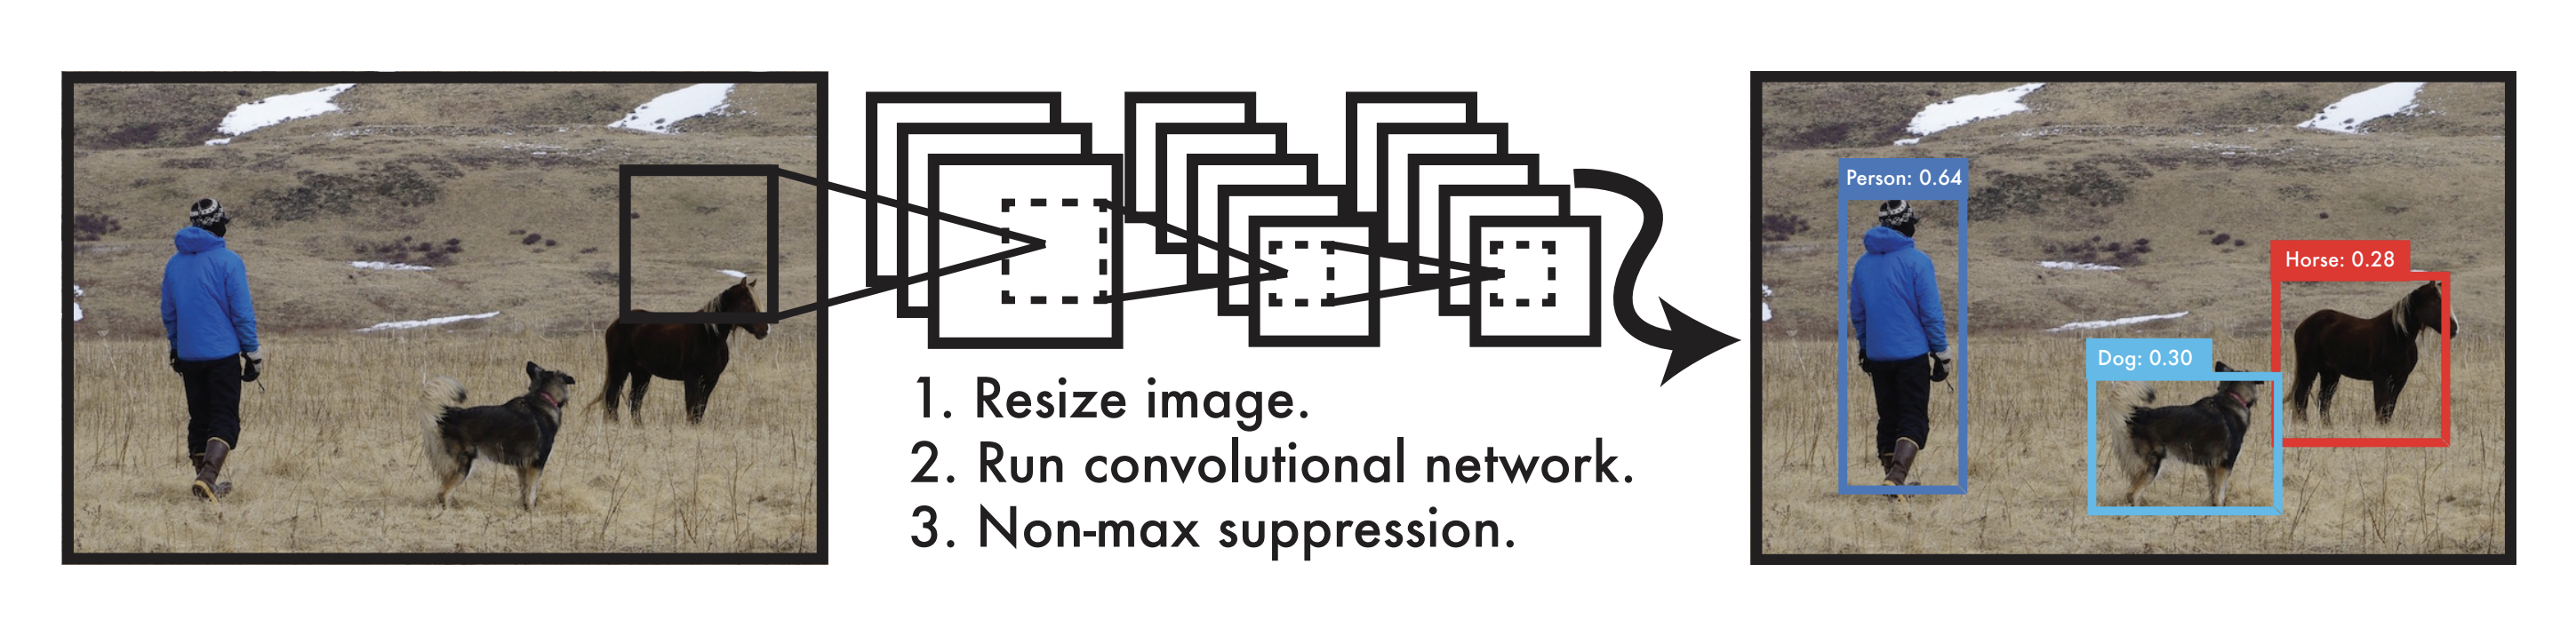
\includegraphics[width=10cm]{yolo_exp.png}
        \caption{The YOLO Detection System.}
        \end{figure}
    \end{document}